% !TeX root = RJwrapper.tex
\title{Changes in R}


\author{by Tomas Kalibera and Sebastian Meyer}

\maketitle

\abstract{%
We present selected changes in the development version of R, which is referred to as R-devel and is to become R 4.5. We also provide some statistics on bug tracking activities in 2024, which covers 4 months before the release of R 4.4 and 8 months of work on R-devel.
}

\section{Selected changes in R-devel}\label{selected-changes-in-r-devel}

R 4.5.0 is due to be released around April 2025. The following gives a
selection of changes in R-devel, which are likely to appear in the new
release.

For a more complete list of changes, run \texttt{news(is.na(Version))} in R-devel or
inspect the nightly rendered version of the \texttt{NEWS.Rd} source file at
\url{https://CRAN.R-project.org/doc/manuals/r-devel/NEWS.html} or its RSS feed at
\url{https://developer.R-project.org/RSSfeeds.html}. The bundled \emph{R~News}
give concise descriptions of a large number of changes, including many
smaller ones.

\subsection{Selected user-visible changes}\label{selected-user-visible-changes}

\begin{itemize}
\item
  R packages for installation are now downloaded in parallel, which improves
  the download speed, on some systems by a large factor.

  Existing support for simultaneous download in \texttt{download.files()} has been
  improved and functions \texttt{install.packages()} and \texttt{download.packages()} now
  use it with the default download method (\texttt{libcurl}). Downloading a single
  file requires a number of handshakes between the client and the server,
  which may be expensive especially on connections with large latencies.
  With simultaneous download, existing connections to the same server may be
  re-used and handshakes be made in parallel with each other and with other
  transfers. The actual speedup depends on network characteristics, but
  significant speedups have been observed both with some very good as well
  as with some rather poor network connections.

  The speedups are bigger when HTTP version 2 is used, which depends on the
  server (many CRAN mirrors support it) and when the curl library used on
  the client supports it (on Unix and macOS it typically does, on Windows
  the upcoming Rtools45 will support it).

  More details about this work can be found in a blog post at
  \url{https://blog.r-project.org/2024/12/02/faster-downloads}. The previous
  implementation of simultaneous download has been improved to be more
  careful about available resources, particularly available file handles.

  The implementation of R internet timeout has been improved to allow
  parallel downloads of many files, though there is a semantic gap between
  an absolute-time timeout in R and simultaneous download, where transfers
  may be delayed by ongoing transfers and various connection assets may be
  re-used between transfers.

  The status reporting for simultaneous transfers in \texttt{download.file()} has
  been improved so that the caller can easily find out which individual
  transfers have succeeded. The simultaneous download can be used directly
  also for other files, not only R packages.
\item
  One can now enter and edit arbitrarily long input lines in the R console on
  Linux and macOS (when the Readline library is used, which is normally the case) and
  in Rterm on Windows. Arbitrarily long input lines can also be used in
  Rgui on Windows, but only the last segment can be edited. In previous
  versions of R, there was a hard-coded limit of about 4K bytes, which
  worked fine for input entered manually, but some users ran into problems
  when pasting generated code. On some systems the input was truncated,
  with Rgui on Windows it could also be corrupted.

  More details about this work can be found in a blog post at
  \url{https://blog.r-project.org/2024/08/30/long-input-lines}. The R parser
  itself is always invoked on a fixed-length prefix of the input. When the
  prefix turns out too short to make any progress parsing, the parser is
  re-started with a longer prefix and the length is potentially unlimited.
  This iterative mechanism is exposed in Rgui on Windows, when the user can
  enter additional segments of the line, but then cannot edit the previous
  segment anymore. Still, several bugs leading to input corruption were
  found during this work and fixed.

  Readline, used on Linux and macOS in R, allows to edit lines of arbitrary
  length, so an intermediate layer has been implemented which provides the
  input to the parser using that iterative mechanism. Rterm on Windows uses
  a rewrite of getline library, which has been extended to support editing
  lines of arbitrary length, and again an intermediate layer has been
  implemented to provide that to the parser.
\item
  Support for the SHA-256 hashing algorithm has been added to R's \pkg{tools}
  package via function \texttt{sha256sum()}. It allows hashing files on disk and
  \texttt{raw} vectors of bytes in memory. The underlying implementation used is
  public domain code written by Ulrich Drepper. SHA-256 from the SHA-2
  family of hash functions is considered more secure than MD5 (\texttt{md5sum()})
  and hence is more appropriate whenever the aim is to detect not only
  accidental data corruption, but also malicious modification. SHA-256 is
  generally slower to compute than MD5 and the checksum is twice as long
  (MD5 is 128-bit). \texttt{md5sum()} has been extended to also support
  computation of a hash of \texttt{raw} vector of bytes in memory, so that it has
  the same interface as \texttt{sha256sum()}.
\item
  R now supports \texttt{zstd} compression. Function \texttt{zstdfile()} has been added
  which allows to create R connections to read from and write to
  zstd-compressed files. One can use zstd compression with serialization
  and there is also some support for zstd compression in the \texttt{tar()} and
  \texttt{untar()} functions. The zstd compression support is currently optional
  in R builds: it is only included when the zstd library is available at
  build time on Unix. On Windows, the zstd library is part of Rtools so zstd
  support is always available.

  With the default tuning options used currently in R, \texttt{zstd} offers
  typically slightly worse compression than \texttt{xz}, but is faster. The
  tradeoffs, however, become different with other tuning options.
\item
  There is a new wrapper function \texttt{grepv(...)}, short hand for
  \texttt{grep(...,\ value\ =\ TRUE)}, to return the matching elements themselves
  rather than their indices.
\item
  A PDF document may include metadata in the so-called \emph{document
  information dictionary}. For instance, PDF documents produced by R's
  \texttt{pdf()} device always set \texttt{"R"} as \texttt{Creator} and by default use
  \texttt{"R\ Graphics\ Output"} as \texttt{Title}. An additional argument \texttt{author} has
  now been added to set the \texttt{Author} entry (omitted by default), possibly
  via \texttt{pdf.options()} in an R profile or init script. Furthermore, the new
  logical arguments \texttt{timestamp} (setting \texttt{CreationDate} and \texttt{ModDate}) and
  \texttt{producer} (\texttt{"R\ \textless{}major\textgreater{}.\textless{}minor\textgreater{}"}) can be set to \texttt{FALSE} to disable the
  corresponding metadata fields. Disabling automatic timestamps simplifies
  tracking uncompressed PDF output in version control systems.
\item
  \texttt{R\ CMD\ check} gains an option \texttt{-\/-run-demo} to check the R scripts in the
  \texttt{demo} directory similar to those in \texttt{tests}. This means demos are run,
  potentially compared to reference output in corresponding \texttt{.Rout.save}
  files, and it is checked that required R packages are declared in the
  \texttt{DESCRIPTION} file. Whereas package tests are not installed by default,
  demos are and are thus exposed to users, so package maintainers should
  ensure they work. The new check option provides an alternative to including
  \texttt{demo()} calls in examples or test scripts.
  Demos may be interactive (e.g., some await a browser response, require
  authentication, or contain instructions for special data or software
  setups) and are sometimes used for computationally intensive examples
  (e.g., replication scripts from associated publications), so \texttt{R\ CMD\ check}
  does not run demo scripts by default (similar to \texttt{\textbackslash{}donttest} examples,
  which are only checked with option \texttt{-\/-run-donttest}).
  Package maintainers could add an explicit condition such as
  \texttt{if\ (!interactive())\ quit()} to demo scripts that require interaction,
  so (occasional) checks with \texttt{-\/-run-demo} can be used to cover the others.

  At the time of writing, 603 (3\%) of 22133 packages on CRAN contained a
  demo directory. Of these packages, 117 used undeclared packages in demo
  scripts. Experiments showed that dozens indeed required an interactive
  user or a special setup, and others did not complete within 90 minutes
  (the chosen timeout on the test system).
  Of the remaining 504 packages, 346 (69\%) produced noteworthy errors:
  a considerable amount of 275 packages failed a demo
  with ``could not find function'' or ``object not found'' errors,
  often simply because the script forgot to attach the own package,
  and sometimes because functionality has been removed in the meantime.
  Remaining issues include coding errors that are catched in recent
  versions of R (e.g., length \textgreater{} 1 conditions), dead URLs, or breakage
  that is likely caused by changes in dependencies.
\end{itemize}

\subsection{Selected low-level changes}\label{selected-low-level-changes}

A number of changes in R-devel --- perhaps more than usual --- are
low-level and invisible to R users, but important for the
reliability and maintainability of R and R packages now and in the future.
Some changes of this kind are listed here.

\begin{itemize}
\item
  Progress has been made on improving the C API for R packages and embedding
  applications. The interface has evolved organically over the years,
  sometimes exposing more than necessary or helpful. With some functions it
  is too easy to make errors leading to segfaults or incorrect results.
  Some functions expose too much internal structure or behavior, which needs
  to be changed occasionally to be able to maintain and improve R itself.

  The interface is defined in the `Writing R Extensions' manual,
  see \texttt{RShowDoc("R-exts")} in your version of R or online at
  \url{https://CRAN.R-project.org/manuals.html}: what is mentioned
  there and is available in installed header files (in directory \texttt{R.home("include")}) is
  in the API. Most internal functions not in the API are ``hidden'' in the
  dynamic libraries, which prevents their accidental use. In R-devel they
  are now hidden also on macOS, previously only on Windows and Linux.

  Some non-API functions currently have to remain unhidden, because they are
  needed by base R packages that are part of the R distribution and are
  maintained with R. The cleanup involved hiding some functions that were
  unnecessarily exposed, replacing some functions with
  safer alternatives, and adding some to the API by documenting them. This
  required cooperation of package authors and was tested and tuned on CRAN
  and Bioconductor packages.

  The `Writing R Extensions' manual has been improved so that
  functions/symbols in the API are explicitly flagged to be in the (regular)
  API, Fortran API (for Fortran code), experimental API (subject to change,
  so users must be prepared to adapt much more than with other categories),
  or embedding API (only for applications embedding R, including front-ends).
  There is now internal functionality in R that can query if a given symbol
  is in the API, which allows stricter checking.
\item
  R includes a number of workarounds for bugs in the iconv library shipped with
  recent versions of macOS. The library is used for encoding conversions,
  e.g., when converting between Latin-1 and UTF-8. Despite most R
  installations today use UTF-8 as the native encoding, such conversions are
  still happening, e.g., for plot labels and when importing historical data
  from legacy file formats.

  The iconv implementation that appeared in macOS 14.0 changed the behavior
  with characters not representable in the target encoding, but also caused
  crashes with legitimate use and caused incorrect conversions (garbage in
  output), which has been detected by R developers and users. The bugs lead
  to incorrect behavior with conversion state reset, with incremental
  conversion of an input stream, and with treating byte-order marks. The
  details can be found in a blog post at
  \url{https://blog.r-project.org/2024/12/11/problems-with-iconv-on-macos}.

  The current CRAN builds of R for macOS use a static build of the iconv
  library that existed in earlier versions of macOS (still truly GNU libiconv
  1.11), so are not yet exposed to these problems. However, users building R
  from source on macOS would run into them if not applying workarounds. R
  4.4 already included some of these workarounds, but R-devel includes more
  and the previous ones have been improved. Also, R-devel fixes a problem
  of interaction between one of the older workarounds and an iconv bug
  causing a problem even in the CRAN builds.

  As iconv would usually be linked dynamically when building R from source,
  the workarounds are based on runtime tests that are executed on first use
  of encoding conversion functions. Hopefully these bugs will eventually be
  fixed upstream in macOS, so that these workarounds can be removed. They
  represent a surprisingly large amount of code.
\item
  The detection of invalid memory accesses caused by attempts to access
  elements of empty vectors has been enabled by default and improved to be
  more robust to different inlining decisions by the compiler. Such an
  access now causes an immediate crash of R and can be easily located using
  a debugger. This is achieved via ``poisoning'': a data pointer to an empty
  R vector is intentionally returned invalid.

  Invalid memory accesses can otherwise lead to crashes later in the
  computation or to incorrect results. As a result of this change, a large
  number of memory access bugs have been found in CRAN packages and reported
  to CRAN maintainers. If packages from other repositories, where regular
  checking against R-devel is not in place, start crashing with R 4.5, this
  is one of the possible causes.

  The amount of related changes in R-devel is small, but the effort
  debugging packages and providing fixes or advice to package maintainers
  has been significant.
\item
  R-devel on Windows has been updated so that it can be built also with some
  alternative Msys2 toolchains, not only with Rtools. This required changes
  in the make files and is based on \texttt{pkg-config}, which is used for figuring
  out library dependencies and C preprocessor options. It simplifies
  testing of the Windows-specific code in R with newer compilers (newer than
  currently in Rtools) and it allows using sanitizers on this code. Also,
  newer compilers with better diagnostics may find problems relevant also
  for the current compilers in Rtools. R-devel has been tested on Windows
  with some of the Msys2 toolchains and sanitizers. In previous years, some
  alternative toolchains have also been tested, but it required ad-hoc
  manual modification of the make files in the R sources.

  This support can also be used for testing package code with alternative
  toolchains, which however requires some Windows-specific knowledge. It is
  essential that all code in use is built by the same toolchain, so for
  these experiments, one needs to start with an empty library. Also, Msys2
  uses dynamic linking, so one can only run (test) the result with the
  corresponding Msys2 toolchain environment. More details are available in
  a blog at
  \url{https://blog.r-project.org/2025/01/28/alternative-toolchains-on-windows}.
\item
  C23 is a new C standard that brings several new features to the language,
  including \texttt{bool}, \texttt{true} and \texttt{false} keywords. It is the default standard
  used by GCC 15, which is expected to be released as stable around the
  release of R 4.5 . R-devel, as well as the upcoming third patch release of R
  4.4, has been made installable with the current pre-release version of GCC
  15 and also with older compilers when the C23 standard is selected
  explicitly.

  R packages affected by this change may either choose to explicitly require
  some older C standard (possibly C17), or better be updated to work also
  with C23. R-devel has been switched to use C23 always when the compiler
  supports it, even when it is not the default standard of the compiler.
  This change has been tested on CRAN and Bioconductor packages and fixes
  were provided to the maintainers.

  In addition to the general need of updating code to newer standards so
  that it can be maintained in the future (say, when other components, e.g.,
  libraries, would use newer standards), some of the C23 features may be useful in R,
  such as the \texttt{bool} type. See `Writing R Extensions',
  Section 1.2.5 (\href{https://CRAN.R-project.org/doc/manuals/r-devel/R-exts.html\#C-standards}{online version}),
  for more details on the use of C standards with R.
\item
  Further progress has been made on getting rid of symbol remapping, i.e.,
  automated renaming of C symbols like \texttt{allocVector()} to \texttt{Rf\_allocVector()}
  done by R headers. The remapping causes problems when it accidentally
  modifies code included via C preprocessor headers. The risks can be
  minimized by including headers in a certain order, but it is an additional
  constraint package authors need to think about, and in practice, the
  conflicts are a common cause of package compilation errors arising after
  updates of the toolchain, OS, or a library.

  The remapping in R-devel has been disabled for C++ code in packages,
  because most of the conflicts happened to be found with C++ code. The
  remapping still remains available and is done by default for C code, but
  it is recommended not to use the remapping in new C code. The `Writing R
  Extensions' manual has been updated to use full names of the functions
  including the prefixes; see Section 6 (``The R API'',
  \href{https://CRAN.R-project.org/doc/manuals/r-devel/R-exts.html\#The-R-API}{online version}),
  for more details on the re-mapping situation in R-devel.

  Similarly, ``strict R headers'' are now the default, which means that legacy
  definitions of \texttt{Calloc}, \texttt{Realloc}, \texttt{Free} and \texttt{PI} have been removed. One
  can still use these allocation functions with the \texttt{R\_} prefix, and \texttt{M\_PI} is a
  standard replacement for \texttt{PI}.

  Like with other similar tasks, this required only relatively small changes
  in R itself, but most of the effort has been spent on testing with CRAN
  and Bioconductor packages and helping the package maintainers with the
  necessary updates.
\end{itemize}

\section{Bug statistics for 2024}\label{bug-statistics-for-2024}

Summaries of bug-related activities over the past year were derived from the
database underlying \href{https://bugs.R-project.org/}{R's Bugzilla system}.
Overall, 183 new bugs or feature requests (15\%) were submitted in 2024,
very much like in the previous two years.
The top 5 selected components for these reports were
``Documentation'', ``Low-level'', ``Misc'', ``Language'', and ``Graphics'',
where the first and last increased their rank compared to 2023.

A total of 107 contributors added 742 comments on 250 different reports; 149
reports were closed. Whereas the number of new submissions remained at
the same level, open issues were handled at a slower rate compared to 2023,
with a decrease in the numbers of closures (--27\%), comments (--21\%), and
contributors (--11\%). Compared to 2022, there is also a decrease in bug
closures and comments, but it is smaller (--13\% closures, --15\% comments,
--13\% contributors).

The numbers of comments and different contributors in the bug tracking system
may be influenced by `R Dev Days' organized by the \href{https://contributor.R-project.org/}{R Contribution Working
Group}: the bugs are pre-discussed at
those events mostly outside the core system, which later receives summarized
comments. An `R Dev Day' organized just after
UseR 2024 had 8 R Core Team members present, so some ``comments'' were exchanged
in person.

The monthly numbers shown in Figure \ref{fig:bzstats-mon} suggest that more
issues were closed in April/May, July/August and November. April/May was
around the release of R 4.4, but also one of the `R Dev Days' took place.
July/August covers the UseR! 2024 conference with an attached R Core Team
meeting and `R Dev Day'.

As every year, not all bug reports go through R Bugzilla. Some are picked
up from the R-devel, R-pkg-devel or R-help mailing lists. Some come via
private communication by e-mail or in person. A number of bugs are always
discovered by the R Core Team when testing changes in R or packages; these
bugs are usually not reported by any channel, but are fixed directly.

\begin{figure}

{\centering 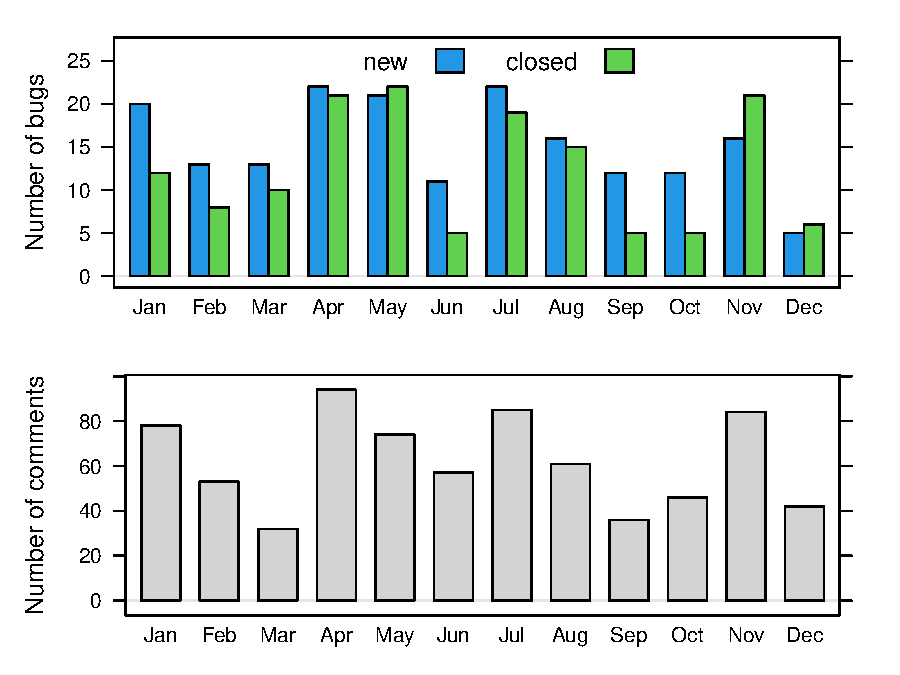
\includegraphics[width=0.8\linewidth,alt={Barplots of the number of opened bugs, closed bugs and comments by month.}]{figures/bzstats-mon} 

}

\caption{Bug tracking activity by month in 2024.}\label{fig:bzstats-mon}
\end{figure}


\address{%
Tomas Kalibera\\
R Core Team\\%
Prague, Czechia\\
%
%
\textit{ORCiD: \href{https://orcid.org/0000-0002-7435-734X}{0000-0002-7435-734X}}\\%
\href{mailto:Tomas.Kalibera@R-project.org}{\nolinkurl{Tomas.Kalibera@R-project.org}}%
}

\address{%
Sebastian Meyer\\
Friedrich-Alexander-Universität Erlangen-Nürnberg\\%
Erlangen, Germany\\
%
%
\textit{ORCiD: \href{https://orcid.org/0000-0002-1791-9449}{0000-0002-1791-9449}}\\%
\href{mailto:Sebastian.Meyer@R-project.org}{\nolinkurl{Sebastian.Meyer@R-project.org}}%
}
